\section{Эксперементальная часть}

Входнные данные:
\begin{enumerate}
	\item a = 1, b = 10;
	\item x = 5, lam = 16;
	\item $\triangle$t = 1
	\item Заявки 10, 100, 1000, 10000;
	\item Минимальная длина очереди = 10;
\end{enumerate}

\subsection{Примеры работы}

% TODO: \usepackage{graphicx} required
\begin{figure}[h]
	\centering
	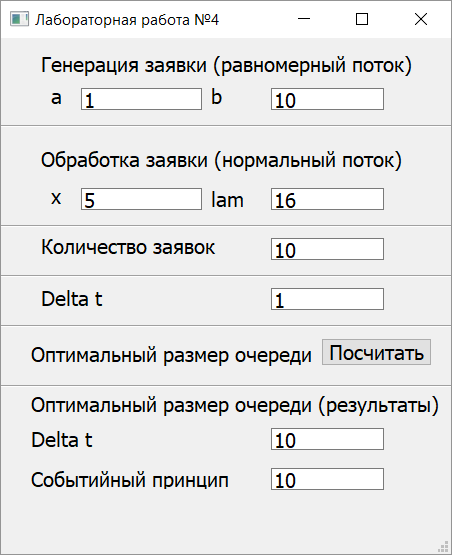
\includegraphics[width=0.7\linewidth]{src/resut_10}
	\caption{Количество заявок: 10}
	\label{fig:resut10}
\end{figure}

% TODO: \usepackage{graphicx} required
\begin{figure}[h]
	\centering
	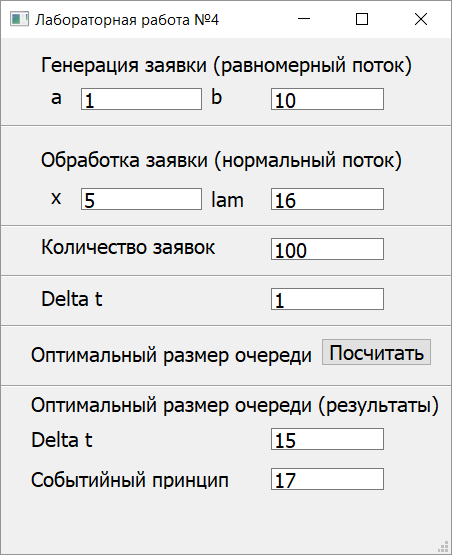
\includegraphics[width=0.7\linewidth]{src/resutl_100}
	\caption{Количество заявок: 100}
	\label{fig:resutl100}
\end{figure}

% TODO: \usepackage{graphicx} required
\begin{figure}
	\centering
	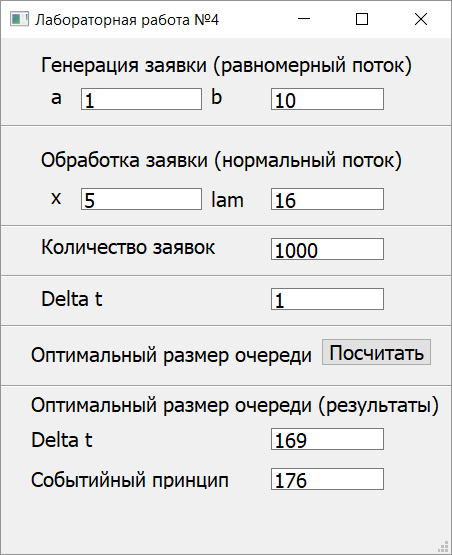
\includegraphics[width=0.7\linewidth]{src/result_1000}
	\caption{Количество заявок: 1000}
	\label{fig:result1000}
\end{figure}

% TODO: \usepackage{graphicx} required
\begin{figure}
	\centering
	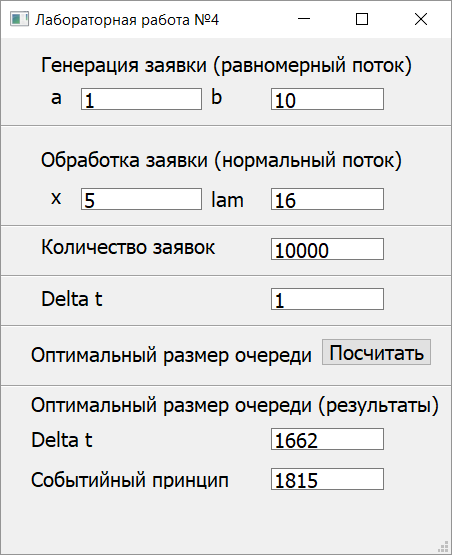
\includegraphics[width=0.7\linewidth]{src/result_100000}
	\caption{Количество заявок: 10000}
	\label{fig:result100000}
\end{figure}


